\documentclass{article}\usepackage[]{graphicx}\usepackage[]{xcolor}
% maxwidth is the original width if it is less than linewidth
% otherwise use linewidth (to make sure the graphics do not exceed the margin)
\makeatletter
\def\maxwidth{ %
  \ifdim\Gin@nat@width>\linewidth
    \linewidth
  \else
    \Gin@nat@width
  \fi
}
\makeatother

\definecolor{fgcolor}{rgb}{0.345, 0.345, 0.345}
\newcommand{\hlnum}[1]{\textcolor[rgb]{0.686,0.059,0.569}{#1}}%
\newcommand{\hlsng}[1]{\textcolor[rgb]{0.192,0.494,0.8}{#1}}%
\newcommand{\hlcom}[1]{\textcolor[rgb]{0.678,0.584,0.686}{\textit{#1}}}%
\newcommand{\hlopt}[1]{\textcolor[rgb]{0,0,0}{#1}}%
\newcommand{\hldef}[1]{\textcolor[rgb]{0.345,0.345,0.345}{#1}}%
\newcommand{\hlkwa}[1]{\textcolor[rgb]{0.161,0.373,0.58}{\textbf{#1}}}%
\newcommand{\hlkwb}[1]{\textcolor[rgb]{0.69,0.353,0.396}{#1}}%
\newcommand{\hlkwc}[1]{\textcolor[rgb]{0.333,0.667,0.333}{#1}}%
\newcommand{\hlkwd}[1]{\textcolor[rgb]{0.737,0.353,0.396}{\textbf{#1}}}%
\let\hlipl\hlkwb

\usepackage{framed}
\makeatletter
\newenvironment{kframe}{%
 \def\at@end@of@kframe{}%
 \ifinner\ifhmode%
  \def\at@end@of@kframe{\end{minipage}}%
  \begin{minipage}{\columnwidth}%
 \fi\fi%
 \def\FrameCommand##1{\hskip\@totalleftmargin \hskip-\fboxsep
 \colorbox{shadecolor}{##1}\hskip-\fboxsep
     % There is no \\@totalrightmargin, so:
     \hskip-\linewidth \hskip-\@totalleftmargin \hskip\columnwidth}%
 \MakeFramed {\advance\hsize-\width
   \@totalleftmargin\z@ \linewidth\hsize
   \@setminipage}}%
 {\par\unskip\endMakeFramed%
 \at@end@of@kframe}
\makeatother

\definecolor{shadecolor}{rgb}{.97, .97, .97}
\definecolor{messagecolor}{rgb}{0, 0, 0}
\definecolor{warningcolor}{rgb}{1, 0, 1}
\definecolor{errorcolor}{rgb}{1, 0, 0}
\newenvironment{knitrout}{}{} % an empty environment to be redefined in TeX

\usepackage{alltt}
\usepackage[margin=1.0in]{geometry} % To set margins
\usepackage{amsmath}  % This allows me to use the align functionality.
                      % If you find yourself trying to replicate
                      % something you found online, ensure you're
                      % loading the necessary packages!
\usepackage{amsfonts} % Math font
\usepackage{fancyvrb}
\usepackage{hyperref} % For including hyperlinks
\usepackage[shortlabels]{enumitem}% For enumerated lists with labels specified
                                  % We had to run tlmgr_install("enumitem") in R
\usepackage{float}    % For telling R where to put a table/figure
\usepackage{natbib}        %For the bibliography
\bibliographystyle{apalike}%For the bibliography
\IfFileExists{upquote.sty}{\usepackage{upquote}}{}
\begin{document}

\begin{enumerate}
%%%%%%%%%%%%%%%%%%%%%%%%%%%%%%%%%%%%%%%%%%%%%%%%%%%%%%%%%%%%%%%%%%%%%%%%%%%%%%%%
%%%%%%%%%%%%%%%%%%%%%%%%%%%%%%%%%%%%%%%%%%%%%%%%%%%%%%%%%%%%%%%%%%%%%%%%%%%%%%%%
% QUESTION 1
%%%%%%%%%%%%%%%%%%%%%%%%%%%%%%%%%%%%%%%%%%%%%%%%%%%%%%%%%%%%%%%%%%%%%%%%%%%%%%%%
%%%%%%%%%%%%%%%%%%%%%%%%%%%%%%%%%%%%%%%%%%%%%%%%%%%%%%%%%%%%%%%%%%%%%%%%%%%%%%%%
\item Let's create some aRt! 
\begin{enumerate}
%%%%%%%%%%%%%%%%%%%%%%%%%%%%%%%%%%%%%%%%%%%%%%%%%%%%%%%%%%%%%%%%%%%%%%%%%%%%%%%%
% QUESTION 1a
%%%%%%%%%%%%%%%%%%%%%%%%%%%%%%%%%%%%%%%%%%%%%%%%%%%%%%%%%%%%%%%%%%%%%%%%%%%%%%%%
  \item Install the \texttt{aRtsy} package. Provide the code in an R chunk that does 
  not run. You only need to install it one time.\\
\textbf{Solution:}
% Note that I have added eval=FALSE so that it won't run
% each time I compile
\begin{knitrout}\scriptsize
\definecolor{shadecolor}{rgb}{0.969, 0.969, 0.969}\color{fgcolor}\begin{kframe}
\begin{alltt}
\hlcom{# Code to install the aRtsy package}
\hlkwd{install.packages}\hldef{(}\hlsng{"aRtsy"}\hldef{)}
\end{alltt}
\end{kframe}
\end{knitrout}
%%%%%%%%%%%%%%%%%%%%%%%%%%%%%%%%%%%%%%%%%%%%%%%%%%%%%%%%%%%%%%%%%%%%%%%%%%%%%%%%
% QUESTION 1b
%%%%%%%%%%%%%%%%%%%%%%%%%%%%%%%%%%%%%%%%%%%%%%%%%%%%%%%%%%%%%%%%%%%%%%%%%%%%%%%%
  \item Load the \texttt{aRtsy} package. Provide the code in an R chunk that does run. 
  We need to load the library each time it is run.\\
\textbf{Solution:}
% Note here I have removed eval=FALSE so this code will run
\begin{knitrout}\scriptsize
\definecolor{shadecolor}{rgb}{0.969, 0.969, 0.969}\color{fgcolor}\begin{kframe}
\begin{alltt}
\hlkwd{library}\hldef{(}\hlsng{'aRtsy'}\hldef{)}
\end{alltt}
\end{kframe}
\end{knitrout}
%%%%%%%%%%%%%%%%%%%%%%%%%%%%%%%%%%%%%%%%%%%%%%%%%%%%%%%%%%%%%%%%%%%%%%%%%%%%%%%%
% QUESTION 1c
%%%%%%%%%%%%%%%%%%%%%%%%%%%%%%%%%%%%%%%%%%%%%%%%%%%%%%%%%%%%%%%%%%%%%%%%%%%%%%%%
 \item Running \texttt{demo("aRtsy")} or \texttt{vignette("aRtsy")} don't return 
 any helpful demos or tutorials. However, if you run \texttt{help("aRtsy")} you 
 will find a link to a tutorial. Recreate the first figure they make using 
 \texttt{canvas\_collatz()}. Make sure to update the caption.\\
\textbf{Solution:}
\begin{knitrout}\scriptsize
\definecolor{shadecolor}{rgb}{0.969, 0.969, 0.969}\color{fgcolor}\begin{kframe}
\begin{alltt}
\hlcom{# help("aRtsy")}
\hlkwd{set.seed}\hldef{(}\hlnum{1}\hldef{)}
\hlkwd{canvas_collatz}\hldef{(}\hlkwc{colors} \hldef{=} \hlkwd{colorPalette}\hldef{(}\hlsng{"tuscany3"}\hldef{))}
\end{alltt}
\end{kframe}
\end{knitrout}
%Code to insert a figure [H]ere
\begin{figure}[H]
\begin{center}
\begin{knitrout}
\definecolor{shadecolor}{rgb}{0.969, 0.969, 0.969}\color{fgcolor}
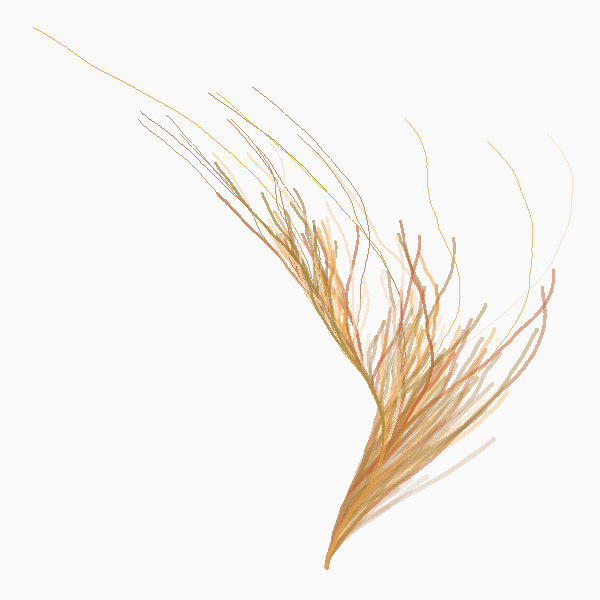
\includegraphics[width=\maxwidth]{figure/unnamed-chunk-3-1} 
\end{knitrout}
\caption{Figure made using \texttt{canvas\_collatz()}}
\label{CollatzPlot1}
\end{center}
\end{figure}
%%%%%%%%%%%%%%%%%%%%%%%%%%%%%%%%%%%%%%%%%%%%%%%%%%%%%%%%%%%%%%%%%%%%%%%%%%%%%%%%
% QUESTION 1d
%%%%%%%%%%%%%%%%%%%%%%%%%%%%%%%%%%%%%%%%%%%%%%%%%%%%%%%%%%%%%%%%%%%%%%%%%%%%%%%%
  \item Change the randomization seed to 1313, which will change the random
  numbers generated to create the plot. Can you see the difference? Make sure to 
  update the caption.\\
\textbf{Solution:}
\begin{knitrout}\scriptsize
\definecolor{shadecolor}{rgb}{0.969, 0.969, 0.969}\color{fgcolor}\begin{kframe}
\begin{alltt}
\hlkwd{set.seed}\hldef{(}\hlnum{1313}\hldef{)}
\hlkwd{canvas_collatz}\hldef{(}\hlkwc{colors} \hldef{=} \hlkwd{colorPalette}\hldef{(}\hlsng{"tuscany3"}\hldef{))}
\end{alltt}
\end{kframe}
\end{knitrout}
%Code to insert a figure [H]ere
\begin{figure}[H]
\begin{center}
\begin{knitrout}
\definecolor{shadecolor}{rgb}{0.969, 0.969, 0.969}\color{fgcolor}
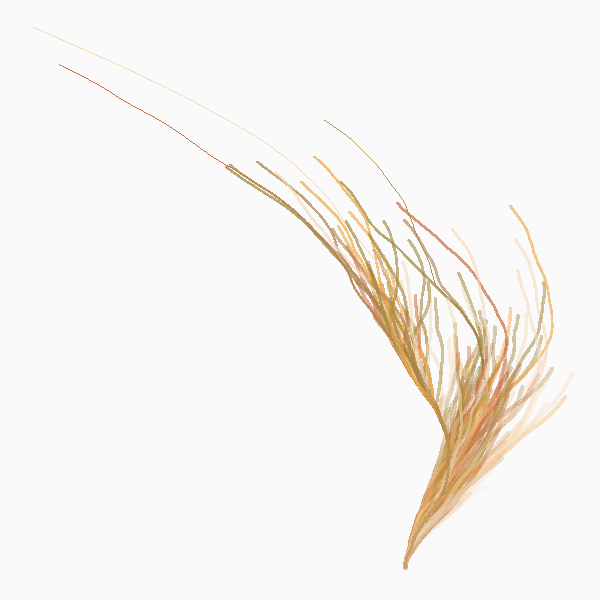
\includegraphics[width=\maxwidth]{figure/unnamed-chunk-4-1} 
\end{knitrout}
\caption{Random seed is 1313, the branches of the graph appear closer together}
\label{CollatzPlot2}
\end{center}
\end{figure}
%%%%%%%%%%%%%%%%%%%%%%%%%%%%%%%%%%%%%%%%%%%%%%%%%%%%%%%%%%%%%%%%%%%%%%%%%%%%%%%%
% QUESTION 1e
%%%%%%%%%%%%%%%%%%%%%%%%%%%%%%%%%%%%%%%%%%%%%%%%%%%%%%%%%%%%%%%%%%%%%%%%%%%%%%%%
  \item Now, create a new Collatz conjecture plot by specifying the following 
  arguments. Note you will find the help file for the \texttt{canvas\_collatz()} 
  function to be rather helpful. Make sure to update the caption.
  \begin{itemize}
  \item Use the \texttt{vrolik4} color palette. Note you can find other by running 
  \texttt{?colorPalette} in the console.
  \item Make the background grey. Note a hexcode for grey is \texttt{\#dbdbdb}.
  \item Specify that there should be 72 strands.
  \item Specify the angle used for bending the sequence for odd numbers as -0.05.
  \item Specify the angle used for bending the sequence for even numbers as 0.0145 
  (note this is the default).
  \end{itemize}
\textbf{Solution:}
\begin{knitrout}\scriptsize
\definecolor{shadecolor}{rgb}{0.969, 0.969, 0.969}\color{fgcolor}\begin{kframe}
\begin{alltt}
\hlkwd{set.seed}\hldef{(}\hlnum{1}\hldef{)}
\hlkwd{canvas_collatz}\hldef{(}
  \hlkwc{colors} \hldef{=} \hlkwd{colorPalette}\hldef{(}\hlsng{"vrolik4"}\hldef{),}
  \hlkwc{background} \hldef{=} \hlsng{'#dbdbdb'}\hldef{,}
  \hlkwc{n} \hldef{=} \hlnum{72}\hldef{,}
  \hlkwc{angle.odd} \hldef{=} \hlopt{-}\hlnum{0.05}\hldef{,}
  \hlkwc{angle.even} \hldef{=} \hlnum{0.0145}\hldef{)}
\end{alltt}
\end{kframe}
\end{knitrout}
%Code to insert a figure [H]ere
\begin{figure}[H]
\begin{center}
\begin{knitrout}
\definecolor{shadecolor}{rgb}{0.969, 0.969, 0.969}\color{fgcolor}
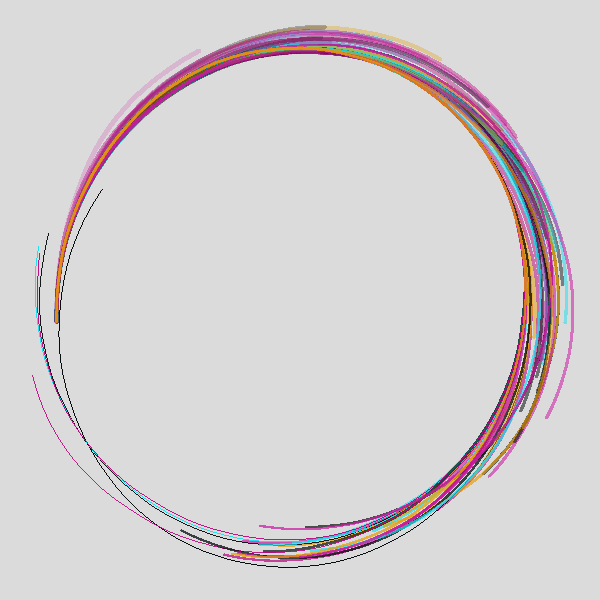
\includegraphics[width=\maxwidth]{figure/unnamed-chunk-5-1} 
\end{knitrout}
\caption{Plot with specified arguments}
\label{CollatzPlot3}
\end{center}
\end{figure}
%%%%%%%%%%%%%%%%%%%%%%%%%%%%%%%%%%%%%%%%%%%%%%%%%%%%%%%%%%%%%%%%%%%%%%%%%%%%%%%%
% QUESTION 1f
%%%%%%%%%%%%%%%%%%%%%%%%%%%%%%%%%%%%%%%%%%%%%%%%%%%%%%%%%%%%%%%%%%%%%%%%%%%%%%%%
  \item Make another plot using the tutorial -- feel free to be creative here! 
  Note that I leave creating the R chunk and figure environment to you here. 
  Make sure that your code is well-formatted and your plot is appropriately scaled.\\
  \textbf{Solution:}
\begin{knitrout}\scriptsize
\definecolor{shadecolor}{rgb}{0.969, 0.969, 0.969}\color{fgcolor}\begin{kframe}
\begin{alltt}
\hlkwd{set.seed}\hldef{(}\hlnum{1}\hldef{)}
\hlkwd{canvas_smoke}\hldef{(}\hlkwc{colors} \hldef{=} \hlkwd{colorPalette}\hldef{(}\hlsng{"blossom"}\hldef{),}
             \hlkwc{shape} \hldef{=} \hlkwd{c}\hldef{(}\hlsng{"clouds"}\hldef{),}
             \hlkwc{algorithm} \hldef{=} \hlkwd{c}\hldef{(}\hlsng{"average"}\hldef{))}
\end{alltt}
\end{kframe}
\end{knitrout}
\begin{figure}[H]
\begin{center}
\begin{knitrout}
\definecolor{shadecolor}{rgb}{0.969, 0.969, 0.969}\color{fgcolor}
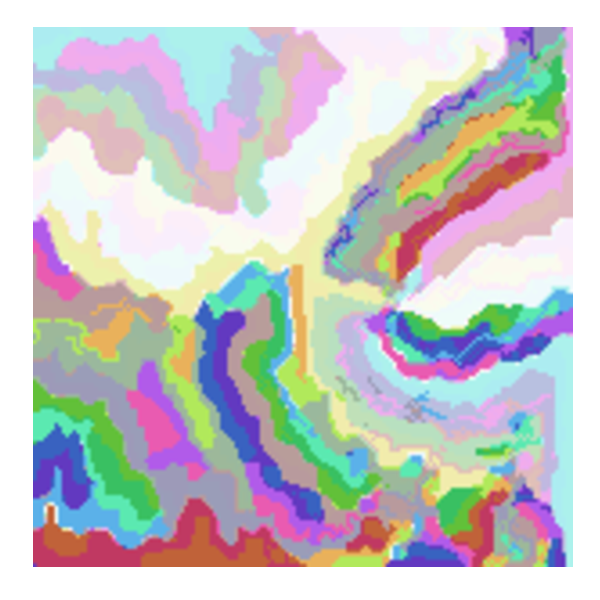
\includegraphics[width=\maxwidth]{figure/unnamed-chunk-6-1} 
\end{knitrout}
\caption{Plot created using \texttt{canvas\_smoke}}
\label{CollatzPlot4}
\end{center}
\end{figure}
%%%%%%%%%%%%%%%%%%%%%%%%%%%%%%%%%%%%%%%%%%%%%%%%%%%%%%%%%%%%%%%%%%%%%%%%%%%%%%%%
% QUESTION 1g
%%%%%%%%%%%%%%%%%%%%%%%%%%%%%%%%%%%%%%%%%%%%%%%%%%%%%%%%%%%%%%%%%%%%%%%%%%%%%%%%
  \item Use \texttt{citation()} to get the BiBTeX citation for the \texttt{aRtsy}
  package and use \verb|\citep{}| to add a parenthetical citation to the end of
  the sentence below.
\textbf{Solution:} We created the generative art in Question 1 using the \texttt{aRtsy}
package for \texttt{R} \citep{artsy}.
\end{enumerate}

\newpage

%%%%%%%%%%%%%%%%%%%%%%%%%%%%%%%%%%%%%%%%%%%%%%%%%%%%%%%%%%%%%%%%%%%%%%%%%%%%%%%%
%%%%%%%%%%%%%%%%%%%%%%%%%%%%%%%%%%%%%%%%%%%%%%%%%%%%%%%%%%%%%%%%%%%%%%%%%%%%%%%%
% QUESTION 2
%%%%%%%%%%%%%%%%%%%%%%%%%%%%%%%%%%%%%%%%%%%%%%%%%%%%%%%%%%%%%%%%%%%%%%%%%%%%%%%%
%%%%%%%%%%%%%%%%%%%%%%%%%%%%%%%%%%%%%%%%%%%%%%%%%%%%%%%%%%%%%%%%%%%%%%%%%%%%%%%%
\item Suppose we wanted to solve $2^{x+1} +2^{x-1} = 40$ for $x$. While this is a pretty straightforward algebra problem, it's useful for demonstrating the use of objects in R. 
  \begin{enumerate}
  %%%%%%%%%%%%%%%%%%%%%%%%%%%%%%%%%%%%%%%%%%%%%%%%%%%%%%%%%%%%%%%%%%%%%%%%%%%%%%%%
  % QUESTION 2a
  %%%%%%%%%%%%%%%%%%%%%%%%%%%%%%%%%%%%%%%%%%%%%%%%%%%%%%%%%%%%%%%%%%%%%%%%%%%%%%%%
  \item Create a numeric vector containing the integers from 0 to 10 inclusive. Hint -- the solution to this problem is one of these values.\\
\textbf{Solution:}
\begin{knitrout}\scriptsize
\definecolor{shadecolor}{rgb}{0.969, 0.969, 0.969}\color{fgcolor}\begin{kframe}
\begin{alltt}
\hldef{num} \hlkwb{<-} \hlkwd{seq}\hldef{(}\hlkwc{from} \hldef{=} \hlnum{0}\hldef{,} \hlkwc{to} \hldef{=} \hlnum{10}\hldef{,} \hlkwc{by} \hldef{=} \hlnum{1}\hldef{)}
\end{alltt}
\end{kframe}
\end{knitrout}
  %%%%%%%%%%%%%%%%%%%%%%%%%%%%%%%%%%%%%%%%%%%%%%%%%%%%%%%%%%%%%%%%%%%%%%%%%%%%%%%%
  % QUESTION 2b
  %%%%%%%%%%%%%%%%%%%%%%%%%%%%%%%%%%%%%%%%%%%%%%%%%%%%%%%%%%%%%%%%%%%%%%%%%%%%%%%%
  \item Complete the algebra to compute $2^{x+1} +2^{x-1}$ for each value in the numerical vector created in step 1. Make sure to save the result to a new numeric vector.\\
\textbf{Solution:}
\begin{knitrout}\scriptsize
\definecolor{shadecolor}{rgb}{0.969, 0.969, 0.969}\color{fgcolor}\begin{kframe}
\begin{alltt}
\hldef{result} \hlkwb{<-} \hlnum{2}\hlopt{^}\hldef{(num}\hlopt{+}\hlnum{1}\hldef{)} \hlopt{+} \hlnum{2}\hlopt{^}\hldef{(num}\hlopt{-}\hlnum{1}\hldef{)}
\end{alltt}
\end{kframe}
\end{knitrout}
  %%%%%%%%%%%%%%%%%%%%%%%%%%%%%%%%%%%%%%%%%%%%%%%%%%%%%%%%%%%%%%%%%%%%%%%%%%%%%%%%
  % QUESTION 2c
  %%%%%%%%%%%%%%%%%%%%%%%%%%%%%%%%%%%%%%%%%%%%%%%%%%%%%%%%%%%%%%%%%%%%%%%%%%%%%%%%
  \item Use the which() function to ask which result is 40.\\
\textbf{Solution:}
\begin{knitrout}\scriptsize
\definecolor{shadecolor}{rgb}{0.969, 0.969, 0.969}\color{fgcolor}\begin{kframe}
\begin{alltt}
\hldef{position} \hlkwb{<-} \hlkwd{which}\hldef{(result}\hlopt{==}\hlnum{40}\hldef{)}
\end{alltt}
\end{kframe}
\end{knitrout}
  %%%%%%%%%%%%%%%%%%%%%%%%%%%%%%%%%%%%%%%%%%%%%%%%%%%%%%%%%%%%%%%%%%%%%%%%%%%%%%%%
  % QUESTION 2d
  %%%%%%%%%%%%%%%%%%%%%%%%%%%%%%%%%%%%%%%%%%%%%%%%%%%%%%%%%%%%%%%%%%%%%%%%%%%%%%%%
  \item What is the solution? That is, what value of x yields $2^{x+1} +2^{x-1} = 40$?\\
\textbf{Solution:}
\begin{knitrout}\scriptsize
\definecolor{shadecolor}{rgb}{0.969, 0.969, 0.969}\color{fgcolor}\begin{kframe}
\begin{alltt}
\hldef{sol} \hlkwb{<-} \hldef{num[position]}
\end{alltt}
\end{kframe}
\end{knitrout}
The solution is 4.
  %%%%%%%%%%%%%%%%%%%%%%%%%%%%%%%%%%%%%%%%%%%%%%%%%%%%%%%%%%%%%%%%%%%%%%%%%%%%%%%%
  % QUESTION 2e
  %%%%%%%%%%%%%%%%%%%%%%%%%%%%%%%%%%%%%%%%%%%%%%%%%%%%%%%%%%%%%%%%%%%%%%%%%%%%%%%%
  \item Explain why this approach wouldn't work for something like $3^{x+2} + 5 (3^x) = 84$ where the solution is $x \approx 1.6309$.\\
\textbf{Solution:}

This approach would not work to find a solution $x$ which is not an integer, because the numeric vector created in step 2a contains only integers (numbers without any decimal value). However, in the example of the problem in 2e, the true solution has decimal value.
\end{enumerate}
\end{enumerate}

\end{document}
